\documentclass[varwidth, border=0pt]{standalone}

\usepackage{times}      % Loads the Times-Roman Fonts
\usepackage{mathptmx}   % Loads the Times-Roman Math Fonts
\usepackage{subcaption}
\usepackage[labelfont={bf,sf},%
labelsep=period,%
justification=centering,
labelformat=parens,labelsep=quad,skip=3pt,font=scriptsize]{caption}
\usepackage{graphicx}

\begin{document}
	
	\begin{figure}
\centering
	\begin{subfigure}{0.5\linewidth}
	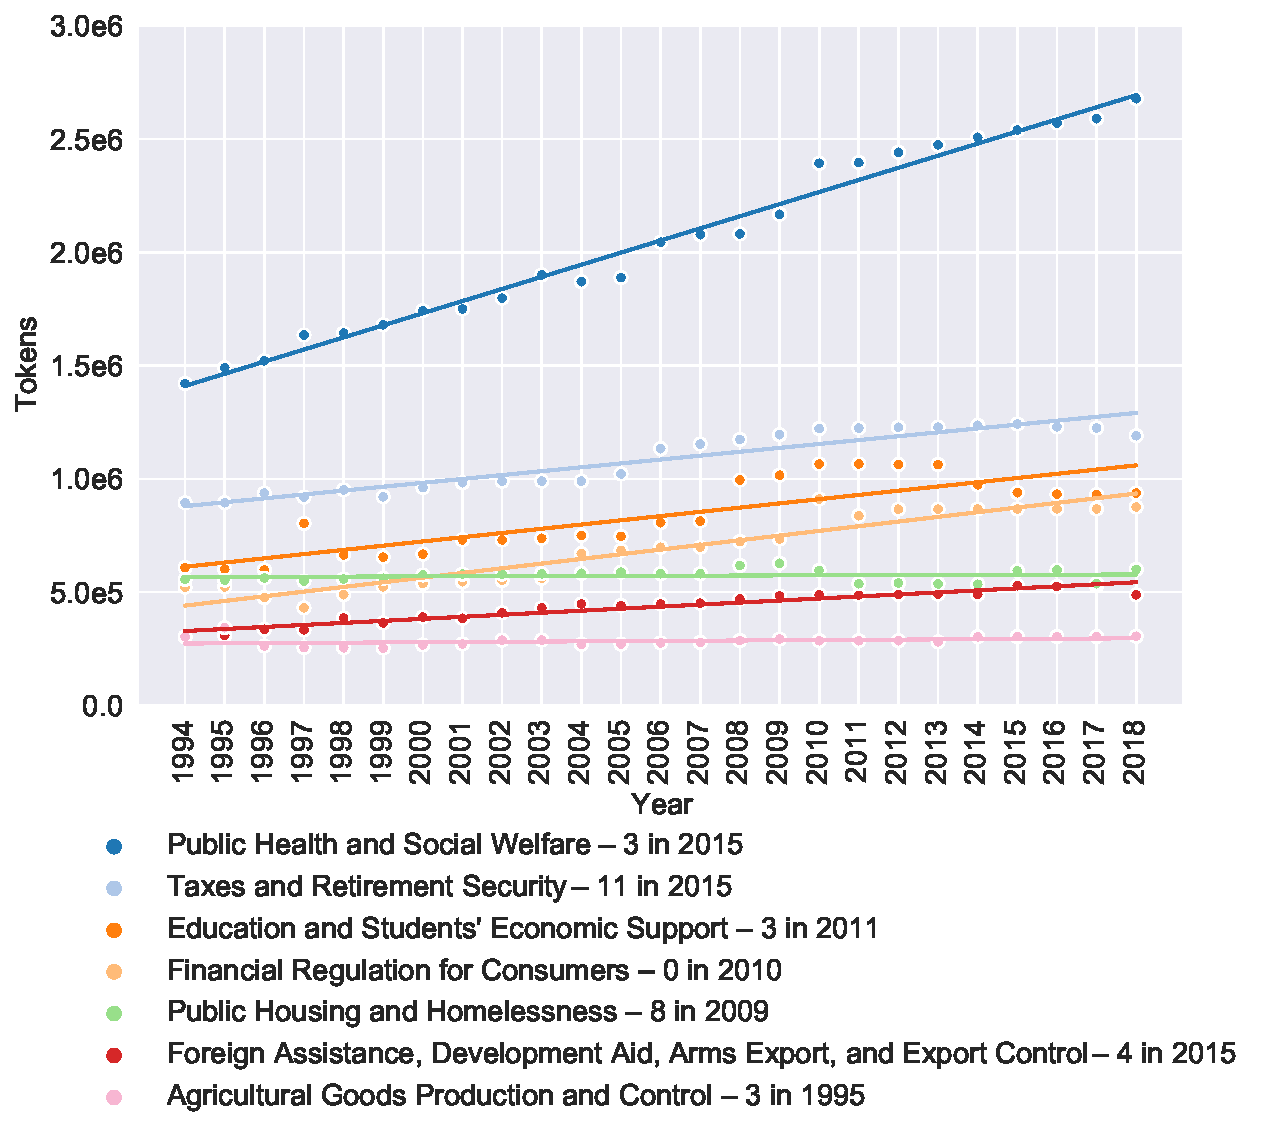
\includegraphics[width=\linewidth]{../../graphics/cluster-evolution-size-dynamics-us-0-0_1-0_-1_a-infomap_n100_m1-0_s0_c1000-selected.pdf}~%
	\subcaption{United States}
\end{subfigure}~%
\begin{subfigure}{0.5\linewidth}
	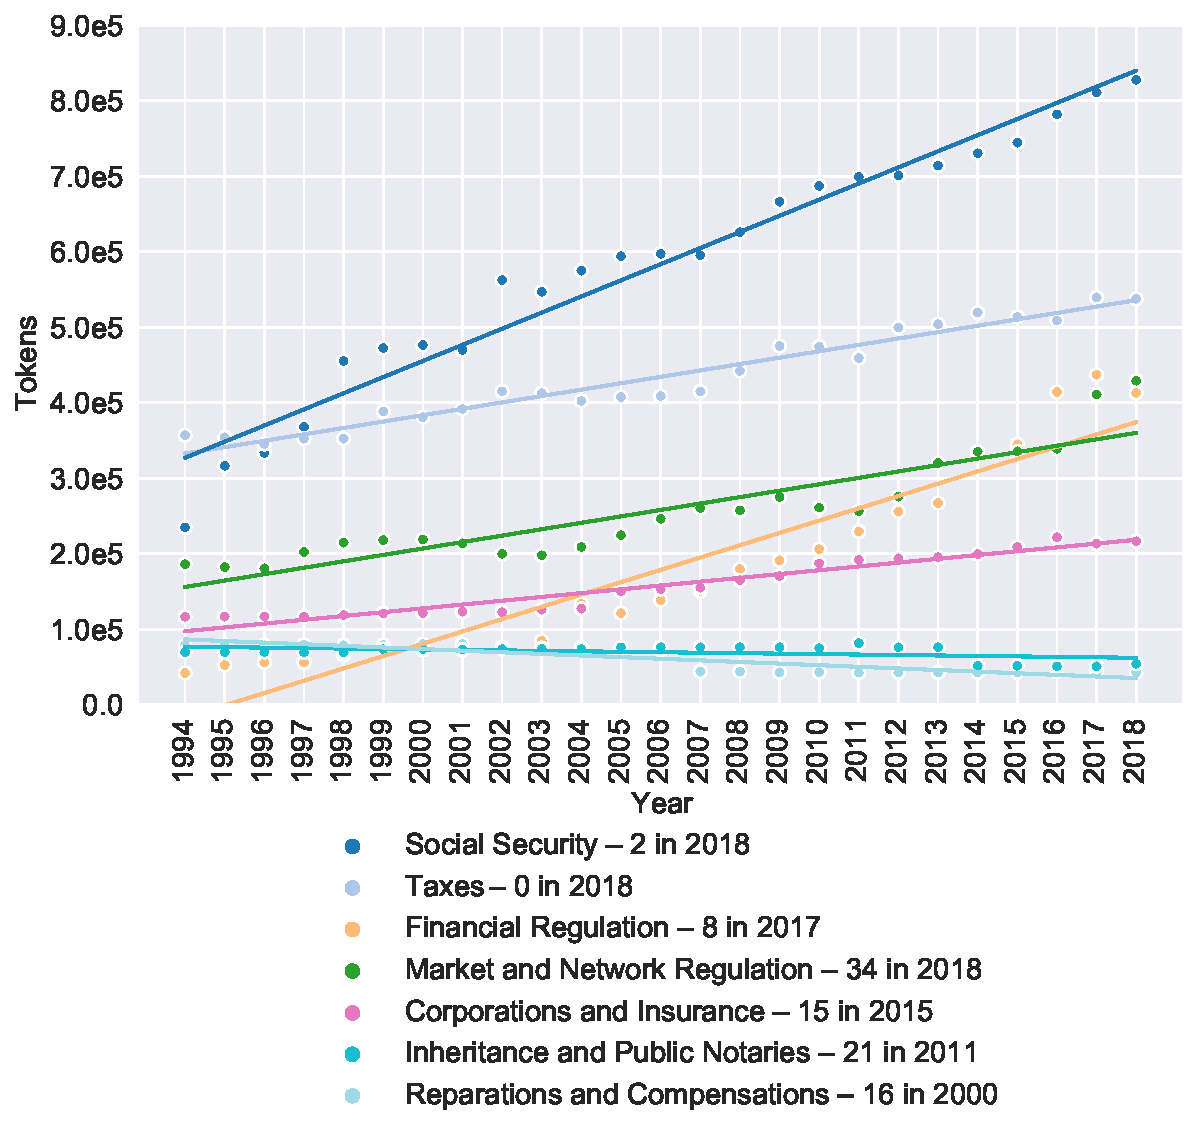
\includegraphics[width=\linewidth]{../../graphics/cluster-evolution-size-dynamics-de-0-0_1-0_-1_a-infomap_n100_m1-0_s0_c1000-selected.pdf}~%
	\subcaption{Germany}
\end{subfigure}
	\end{figure}
	
\end{document}